\documentclass[UTF8]{ctexart}
\usepackage{graphicx}
\usepackage{amsmath}
\pagestyle{plain}   
% \usepackage{booktabs}
% \usepackage{subfigure}
\usepackage{setspace}
\date{}
\title{DataStructureLab0实验报告} 
\author{杨景凯}
\date{2021/3/1} 
\begin{document} 
% \maketitle 
\begin{center}
    \quad \\
    \quad \\
    \quad \\
    \vskip 3.5cm
    \heiti \zihao{1} 哈希表与跳表性能比较\\
\end{center}
\vskip 3.5cm
\begin{quotation}
    \songti \fontsize{30}{30}
    \doublespacing
    \par\setlength\parindent{12em}
    \quad 
\begin{center}
    %学\hspace{0.61cm} 院:\underline{电子信息与电气工程学院}

    学生姓名:\underline{\qquad    \quad \quad 杨景凯    \quad  \quad\qquad }

    学\hspace{0.61cm} 号:\underline{\quad \quad\quad520021910550\quad\quad}

\end{center}
    
    \centering
    2022年3月1日
\end{quotation}
\clearpage
\tableofcontents
\clearpage
\section{理论部分}
\subsection{选择}
我选择跳表。
\subsection{分析}
跳表是在线性结构基础上进行发展的数据结构,它一方面依据随机层数的特性,能够快速查找到数据,另一方面维持了底层线性的特点,更适合于连续数据的遍历。
\section{实验部分}
\subsection{实验说明}
为了证明我的结论,我设计了如下实验。我比较了哈希表、未添加连续搜索函数(只使用简单搜索函数)的跳表和添加了连续搜索函数(连续线性遍历区间元素)的跳表。
实验分为10组,每组区间搜索元素分别为100至1000个。为了更明显地体现差距,将搜索反复进行10000次。输出三种数据结构处理的时间(以秒为单位)。
\subsection{实验结果}
实验结果如下表所示:
\begin{table}[hp]
    \centering
    \textbf{Table of result}
    \begin{tabular}{|c|c|c|c|}
        \hline
        searchtimes& hashtable(s)&	skiplist(add funtion)(s)&	skiplist(not add funtion)(s)\\
        \hline
        100&	0.375&	0.015625&	0.109375\\
        \hline
        200&	0.828125&	0.03125&	0.3125\\
        \hline
        300&	1.26562&	0.03125&	0.453125\\
        \hline
        400&	1.73438&	0.046875&	0.609375\\
        \hline
        500&	2.0625&	0.0625&	0.796875\\
        \hline
        600&	2.375&	0.078125&	0.96875\\
        \hline
        700&	2.82812&	0.078125&	1.09375\\
        \hline
        800&	3.1875&	0.09375&	1.32812\\
        \hline
        900&	3.625&	0.109375&	1.5\\
        \hline
        1000&	4.04688&	0.125&	1.70312\\
        \hline
    \end{tabular}
\end{table}
\newpage
根据实验结果做出的折线图如下:
\begin{center}
    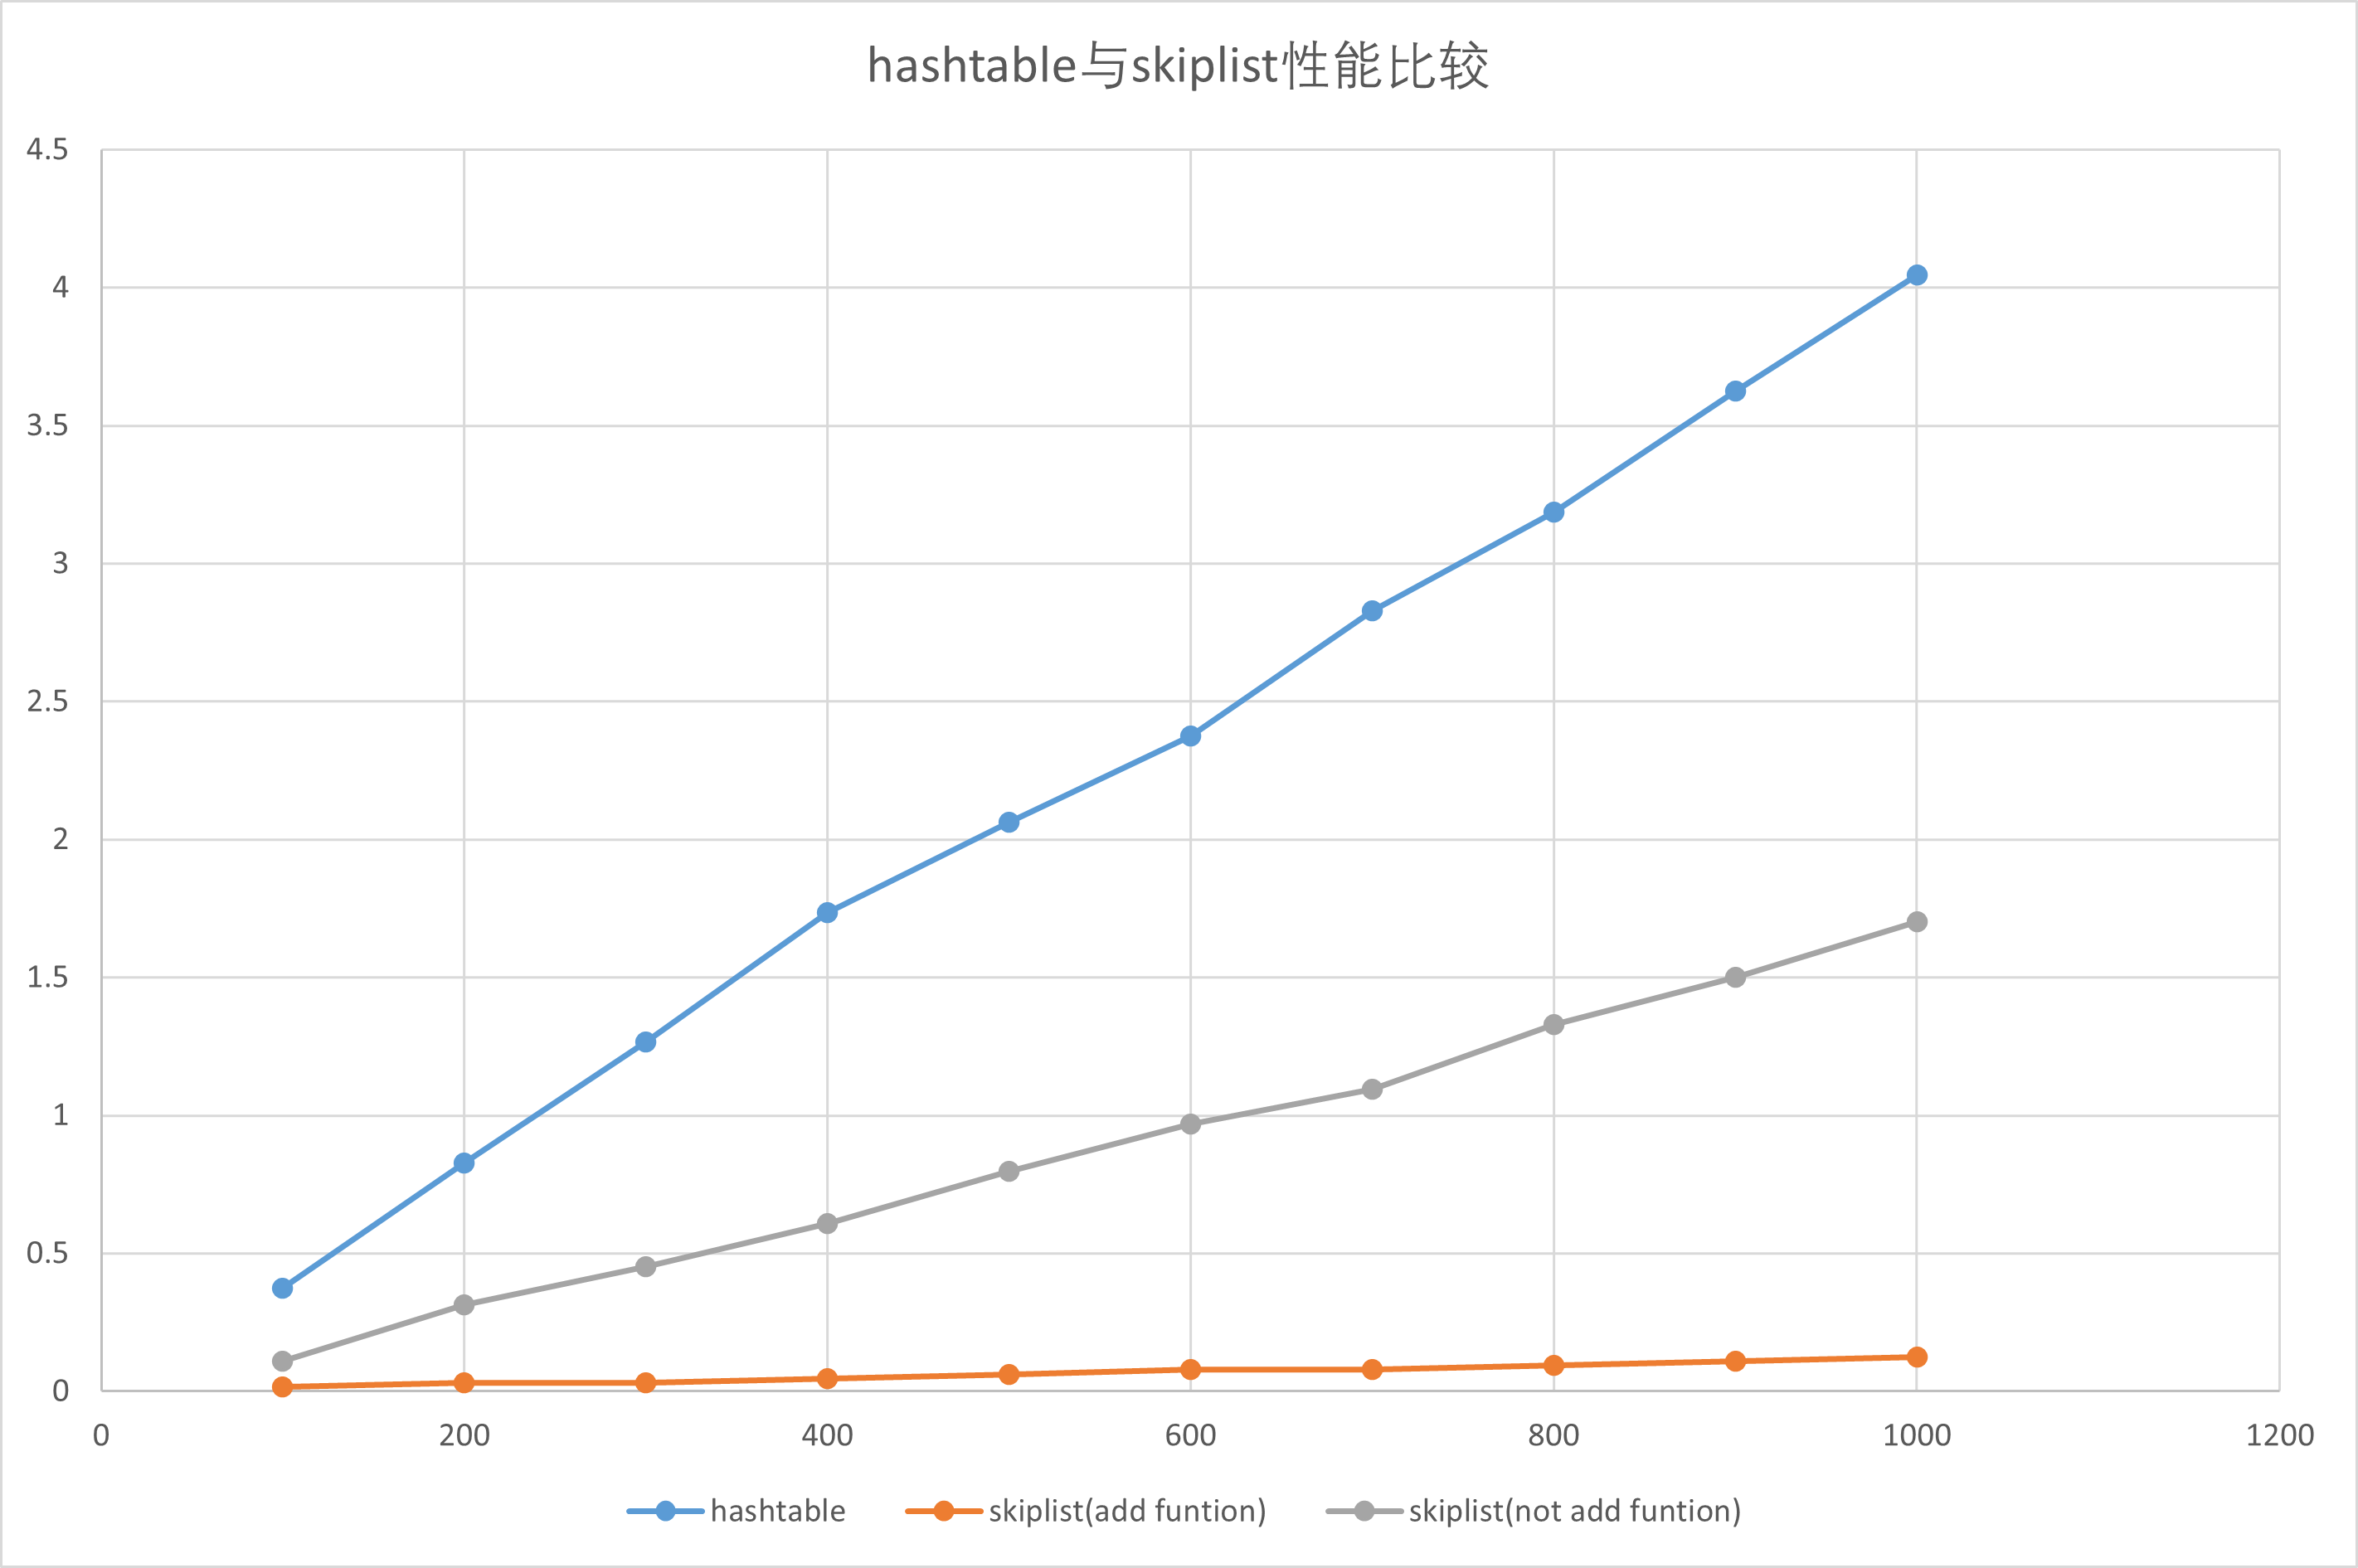
\includegraphics[scale=0.6]{hashtable_and_skiplist.png}
\end{center}
\subsection{实验结论}
根据上述实验,无论是未添加连续搜索函数(只使用简单搜索函数)的跳表还是添加了连续搜索函数(连续线性遍历区间元素)的跳表,在区间搜索性能上都比哈希表要好。因此之前的选择和理论分析正确。


% \clearpage
% \begin{thebibliography}{99} 
% \end{thebibliography}
\end{document}
